\documentclass[11pt,a4paper]{article}
\usepackage[margin=2.2cm]{geometry}
\usepackage[T1]{fontenc}
\usepackage[utf8]{inputenc}
\usepackage{lmodern}
\usepackage{microtype}
\usepackage{graphicx}
\usepackage{booktabs}
\usepackage{adjustbox}
\usepackage{longtable}
\usepackage{array}
\usepackage{float}
\usepackage{xcolor}
\usepackage{enumitem}
\usepackage{amsmath}
\usepackage{xurl}
\usepackage[hidelinks]{hyperref}
\usepackage[nameinlink]{cleveref}
\setlist{nosep,leftmargin=*}
\definecolor{accent}{HTML}{2A78D6}
\hypersetup{colorlinks=true,linkcolor=accent,urlcolor=accent,citecolor=accent}
\setlength{\parskip}{3pt}

\title{\textbf{Four-class LVEF classification from 12-lead ECG printout images}\\[4pt]
\large Complete record of experiments (all branches, Phases 1--7) and final result}
\author{[Student name] \\ Supervisor: [Professor name]}
\date{November 2026}

\begin{document}
\maketitle

\begin{abstract}
\noindent \textbf{Task.} Classify left-ventricular ejection fraction (LVEF) into four classes (Normal, Mild, Moderate,
Severe) from images of hospital 12-lead ECG printouts. Labels come from echocardiography reports (Teichholz EF) linked
to the ECGs by patient-name matching.

\noindent \textbf{Data and protocol.} 837 development ECGs (794 patients) and a locked test set of 210 ECGs.
\begin{itemize}
  \item Every model was evaluated with patient-grouped 5-fold cross-validation repeated 3 times, with all choices
    nested inside the training folds.
  \item Comparisons use corrected repeated-CV tests with Holm correction.
  \item Each study was pre-registered before it was run.
\end{itemize}

\noindent \textbf{What was tested.} Across seven phases and the branches of the repository:
\begin{itemize}
  \item image CNNs, foundation-model embeddings (ECGFounder, ECG-FM) and their fine-tuning;
  \item LSTM, CNN-LSTM and 1-D ResNet models, MiniRocket, median-beat and clinician features;
  \item ensembles, stacking and two-stage models;
  \item label-cleaning schemes, threshold and band sweeps, and an external model trained on about 100,000 patients.
\end{itemize}

\noindent \textbf{Four-class result.} Four-class accuracy on all patients converges at 0.55--0.57 (best image-only
0.571 [0.542, 0.600]; locked test 0.553 [0.485, 0.621]). Mild is the hardest class.

\noindent \textbf{Final model: image-only triage.} It answers only when it is confident and refers the rest to echo.
\begin{itemize}
  \item \textbf{Cross-validation:} 56\,\% of patients answered, with \textbf{0.694} [0.655, 0.736] accuracy.
  \item \textbf{Locked test, scored once:} 50\,\% answered, with \textbf{0.747} [0.660, 0.837] accuracy.
  \item 85--90\,\% of its confident ``Normal'' answers exclude moderate or severe dysfunction.
\end{itemize}

\noindent \textbf{The limit.} The ECG estimates EF to about $\pm$13 points against class bands 10--12 points wide.
Improvement needs ID-linked Simpson EF labels, digital ECGs, more Mild and Moderate patients, or large-scale public
pre-training, which is under way.
\end{abstract}

\tableofcontents
\newpage

% ---------------------------------------------------------------------------------------------------------
\section{Objective}\label{sec:intro}
Estimate the LVEF class of a patient from the image of a standard hospital 12-lead ECG printout:
\begin{itemize}
  \item \textbf{Normal:} EF $>52$\,\% (men) or $\ge54$\,\% (women);
  \item \textbf{Mild:} 41\,\% up to the Normal limit;
  \item \textbf{Moderate:} 31--$<$41\,\%;
  \item \textbf{Severe:} $<31$\,\%.
\end{itemize}
The owner's requirements, as they evolved over the project:
\begin{enumerate}
  \item four-class only (no binary simplification), with the original labels as the primary result;
  \item image only: no printed machine measurements, age or sex as model inputs;
  \item every class detected, with Mild recall $\ge 15$\,\%;
  \item the highest accuracy obtainable without manipulating labels or the evaluation set.
\end{enumerate}

% ---------------------------------------------------------------------------------------------------------
\section{Data}\label{sec:data}
\begin{itemize}
  \item \textbf{ECGs:} 1,047 single-centre 12-lead ECG PDFs from 993 patients (2020--2024: 232 / 294 / 226 / 295),
    in the standard $3\times4$ + rhythm layout. Each lead is 2.5\,s long; lead II also appears as a 10-s rhythm strip.
    Class totals: Normal 480, Mild 232, Moderate 221, Severe 114.
  \item \textbf{Waveforms:} the traces are vector drawings and are digitised exactly from the PDF.
  \item \textbf{Split:}
    \begin{itemize}
      \item a \textbf{development set} of 837 ECGs from 794 patients, used for all modelling;
      \item a \textbf{locked test set} of 210 ECGs from 199 patients, with no patient overlap.
    \end{itemize}
    The original project and Phase 1 scored models on the test split. From Phase 2 on it was locked: never used for
    training or selection, and scored once at the end with the frozen model (Section~\ref{sec:final}).
  \item \textbf{Labels:} Teichholz EF from echocardiography reports, linked to each ECG by fuzzy patient-name
    similarity. The yearly ECG--echo sheets (2020, 2021, 2022, 2024) contain no patient identifier.
  \item \textbf{Development class counts:} Normal 384, Mild 185, Moderate 177, Severe 91.
\end{itemize}

\paragraph{Data-quality audit (Phases 4--6B).}
\begin{itemize}
  \item All 837 development ECGs link to at least one echo.
  \item The folder label agrees with the nearest echo for 93.4\,\% of ECGs (55 disagree).
  \item Link quality: 391 links have a name-match score $<100$; 192 have the nearest echo more than 30 days away.
  \item Echo consistency: 85 ECGs have a linked echo of another class, and 77 have an EF spread of more than 10 points.
  \item 221 ECGs lie within 3 EF points of a class limit.
  \item The 2021 sheet's ECG dates were day/month-swapped; this was corrected (C6A-1) and does not change labels.
  \item 29 near-identical name pairs exist under different patient keys: 15 within development, 11 straddling
    development and test (excluded from the locked-test primary analysis), and 3 within test.
\end{itemize}

% ---------------------------------------------------------------------------------------------------------
\section{Evaluation protocol}\label{sec:protocol}
\begin{itemize}
  \item \textbf{Cross-validation:} patient-grouped 5-fold CV $\times$ 3 repeats, identical folds for every model
    (\texttt{phase\_2/configs/folds\_D.csv}).
  \item \textbf{Nested choices:} hyper-parameters, thresholds and decision rules are chosen only inside the training
    folds (inner CV).
  \item \textbf{Confidence intervals:} corrected repeated-CV 95\,\% CIs (Nadeau--Bengio,
    $n_{\text{train}}=535$, $n_{\text{test}}=167$, 15 cells).
  \item \textbf{Comparisons:} paired corrected $t$-tests with Holm correction. A \emph{genuine improvement} requires
    Holm $p<0.05$, the same sign in all 3 repeats, and admissibility.
  \item \textbf{Admissibility:} every class recall $\ge 0.15$. Eligibility: 3 repeats $\times$ 3 seeds.
  \item \textbf{Pre-registration:} plans and dated amendments were committed before running, so results cannot steer
    the design.
\end{itemize}

% ---------------------------------------------------------------------------------------------------------
\section{Summary of all work}\label{sec:summary}
\begin{table}[H]\centering\small
\caption{Every phase at a glance. Accuracy is four-class: on the test split for the original project and Phase 1,
and in development cross-validation for Phases 2--7. Detail is in Sections~\ref{sec:p15}--\ref{sec:bands}.}\label{tab:summary}
\begin{adjustbox}{max width=\linewidth}
\begin{tabular}{>{\raggedright\arraybackslash}p{2.6cm}>{\raggedright\arraybackslash}p{6.2cm}>{\raggedright\arraybackslash}p{2.8cm}>{\raggedright\arraybackslash}p{4.8cm}}\toprule
Phase & What was tried & Best result & Conclusion \\\midrule
Original & ECGNet, ResNet-18, EfficientNet, MobileNet, ConvNeXt, HOG+SVM, 1-D ResNet, header LR, XGBoost, fusions & 0.552 (header + ResNet-18; test) & the header numbers carried most of the signal; Mild recall 11\,\% \\
Phase 1 & ECGFounder frozen / fine-tuned, ordinal heads, fusions & 0.524, macro-F1 0.448 (A2; test) & foundation model best balanced; test set exposed \\
Phase 2 & audit, pre-registration, development CV, input variants & 0.544 (header + ECGFounder MLP) & rigorous protocol fixed \\
Phase 3 & clinical features, gated / attention fusion, ensembles, calibration & 0.547 (C1 vote) & plateau at 0.53--0.55 \\
Phase 4 & EF regression, multitask, label-quality training & 0.560 (n.s.) & information limit: $r=0.66$ vs 0.80 needed \\
Phase 5 & engineered features, LightGBM, stacking, hierarchy, decision rules, augmentation & \textbf{0.561} (C3, selected) & 0 of 43 genuine improvements \\
Phase 6 & fine-tuning, ECG-FM, inputs, digitisation & 0.561 (unchanged) & no candidate passed the screen \\
Phase 6A/6B & Normal 270, borderline relabelling, T50/T55, Normal sizes, LSTM, CNN-LSTM, fusions & 0.569 (T55, n.s.) & LSTMs significantly worse; definition effects only \\
Label studies & VER, BRES, CLEAR, SUB591, HC30, MMCLEAN, NF, MILDFIX & $\le$ 0.565 on all ECGs & label noise explains $<$\,1 point \\
Phase 7 & multi-scale, soft labels, contrastive, 1-D ResNet, learning curve, cascades & 0.568 (cascade, not admissible) & \textbf{triage 0.694 on 56\,\%} \\
Image-only push & two-stage, 10-s reconstruction, MiniRocket, median beats, stacking, EchoNext-Mini & \textbf{0.571} (ULT-stack) & plateau 0.57; external model adds nothing \\
Band sweep & 3,313 class definitions & 0.626 (ESC 2021) & sensitivity analysis only \\
\textbf{Locked test} & frozen image-only triage model, scored once & \textbf{0.747 on 50\,\%}; 4-class 0.553 & development estimates confirmed \\\bottomrule
\end{tabular}
\end{adjustbox}
\end{table}

% ---------------------------------------------------------------------------------------------------------
\section{Final result: the image-only triage model (the ``69\,\%'' model)}\label{sec:final}

\subsection{Why a triage model}
No model of any family exceeded about 0.57 four-class accuracy on \emph{all} patients
(Sections~\ref{sec:p6}--\ref{sec:bands}). Errors concentrate on ECGs whose echo EF lies near a class limit
(Figure~\ref{fig:boundary}). A model that \emph{answers only when it is confident} and refers the rest to
echocardiography therefore turns the same information into a clinically usable result. The owner chose this framing
(``triage + Mild limitation''). The model was frozen before it was tested.

\subsection{Model definition (frozen 2026-11-06, SHA-256 \texttt{09808d12\ldots})}
\begin{itemize}
  \item \textbf{Input:} the ECG drawing only.
  \begin{itemize}
    \item ECGFounder embedding of the waveform digitised from the PDF;
    \item 118 measurements made on the drawing (clinician-style features);
    \item no printed machine text, no age.
  \end{itemize}
  The patient's sex is used only to place the Normal/Mild cut (52\,\%\ men, 54\,\%\ women), exactly as in the label rule.
  \item \textbf{EF estimate:} the average of a ridge and a LightGBM EF regressor (unverified echo links weighted 0.3).
  \item \textbf{EF grading:} Normal above the sex limit; Mild $45.5$ up to the limit; Moderate $35$--$45.5$; Severe $<35$.
  \item \textbf{Answer rule:} the model answers only when (a) the grade agrees with the image-only four-class
    classifier IMG-C3 (prior rule $\alpha=0.5$), and (b) the EF estimate is at least 3.05 EF points from every cut.
    Otherwise it outputs ``refer to echo''.
  \item \textbf{How the values were chosen:} every threshold was set inside the training folds (nested). The frozen
    copy was refitted on all 837 development ECGs and checked for exact reproduction.
\end{itemize}

\subsection{Results}
\begin{table}[H]\centering\small
\caption{The final image-only model in cross-validation and on the locked test set (scored once,
owner-authorised, 2026-11-06). 95\,\% CIs: corrected repeated-CV (development) and patient-cluster bootstrap (test).}
\label{tab:final}
\begin{adjustbox}{max width=\linewidth}
\begin{tabular}{lcc}\toprule
 & \textbf{Cross-validation} (837 ECGs) & \textbf{Locked test} (199 ECGs) \\\midrule
Triage: share of patients answered & 56\,\% [48, 63] & 49.7\,\% [42.9, 56.7] \\
\textbf{Triage: accuracy on answered patients} & \textbf{0.694} [0.655, 0.736] & \textbf{0.747} [0.660, 0.837] \\
Confident ``Normal'' answers with EF $\ge 41$\,\% & 90\,\% [86, 94] & 85\,\% [77, 92] \\
EF $<41$\,\% patients given a confident ``Normal'' & 15\,\% [8, 22] & 21\,\% [11, 31] \\
Four-class accuracy, all patients (IMG-C3) & 0.558 [0.504, 0.611] & 0.553 [0.485, 0.621] \\
Macro-F1, all patients & 0.441 & 0.453 [0.375, 0.525] \\
Mild precision / recall (all patients) & 0.29 / 0.19 & 0.32 / 0.32 \\\bottomrule
\end{tabular}
\end{adjustbox}
\end{table}

\begin{figure}[H]\centering
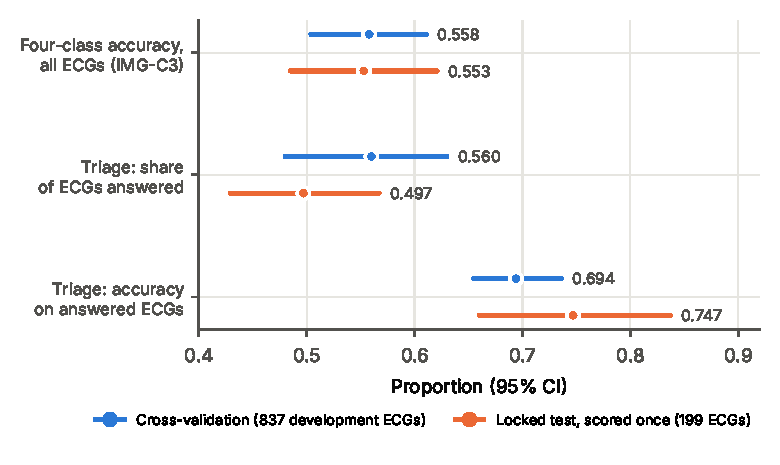
\includegraphics[width=0.78\linewidth]{figures/fig_cv_vs_locked_test.pdf}
\caption{Development estimates carried over to unseen patients: every cross-validation value lies inside its
locked-test confidence interval.}\label{fig:cvtest}
\end{figure}

\begin{figure}[H]\centering
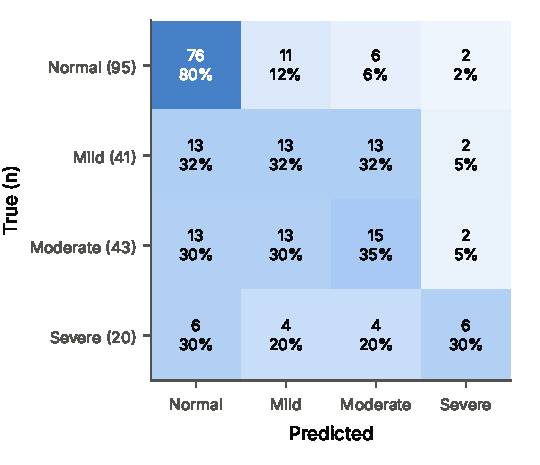
\includegraphics[width=0.5\linewidth]{figures/fig_locked_confusion.pdf}
\caption{Locked-test confusion matrix of the four-class IMG-C3 output (counts and row percentages). Normal is
recognised well; Mild and Moderate are split evenly across Normal, Mild and Moderate.}\label{fig:lockedcm}
\end{figure}

\paragraph{Locked-test details.}
\begin{itemize}
  \item 199 of the 210 locked ECGs form the primary set. 11 were excluded before scoring because their patient key
    forms a near-identical name pair with a development patient.
  \item The 199 ECGs come from 186 patient clusters.
  \item \textbf{Caveat.} The same 210 ECGs had been scored by the original project and in Phase 1 (about 40 models).
    The frozen triage model was developed in Phases 2--7 without any access to them, so the test is independent of its
    development. It is still not a pristine first look at these patients, and a new prospective test set is the
    stronger confirmation.
  \item Triage calls on the locked test: 88 Normal, 10 Moderate, 1 Severe, and no Mild.
  \item Sensitivity analysis on all 210 ECGs: four-class accuracy 0.538; triage 48\,\% answered at 0.743.
\end{itemize}

\subsection{How to state the result}
\begin{quote}
From the ECG image alone, the model gives a confident answer for about half of the patients (56\,\% in
cross-validation, 50\,\% on the locked test), with 0.69--0.75 accuracy on those answers. Most confident answers are
``Normal'', and 85--90\,\% of them exclude moderate or severe LV dysfunction. The remaining patients are referred to
echocardiography. Four-class accuracy on all patients is about 0.55--0.57. Mildly reduced EF cannot be identified
reliably from these printouts.
\end{quote}

\noindent\textbf{Do not claim:}
\begin{itemize}
  \item ``70\,\% accuracy'' without saying \emph{on answered patients} and giving the answered share;
  \item that the triage detects Mild (it made no Mild calls on the locked test);
  \item that it is a stand-alone rule-out: 15--21\,\% of patients with EF $<41$\,\% received a confident ``Normal''.
\end{itemize}
The 210 locked ECGs have now been used, so any further claim needs new ECGs (see the test kit, Appendix~\ref{app:repro}).

% ---------------------------------------------------------------------------------------------------------
\section{Original project and Phases 1--5}\label{sec:p15}

\subsection{Original project (baseline)}
\begin{itemize}
  \item \textbf{Goal:} a CNN on the cropped, grid-filtered ECG page image, predicting the four-class LVEF category
    and a heart-failure yes/no screen.
  \item \textbf{Location:} code on \url{main} (\texttt{ecg\_ef/}); results and write-up on
    \url{claude/funny-gauss-udlmv0}.
  \item \textbf{Evaluation:} scored on the fixed 210-ECG test set.
\end{itemize}
\begin{table}[H]\centering\small
\caption{Original project, fixed test set ($n=210$).}\label{tab:orig}
\begin{adjustbox}{max width=\linewidth}
\begin{tabular}{lccccc}\toprule
Model & Accuracy & Bal.\ acc. & Macro-F1 & QWK & HF AUC \\\midrule
HOG + SVM & 0.481 & 0.322 & 0.283 & 0.229 & 0.737 \\
ECGNet (custom CNN) & 0.471 & 0.360 & 0.262 & 0.389 & 0.745 \\
ResNet-18 (selected image model) & 0.486 & 0.356 & 0.323 & 0.290 & 0.735 \\
EfficientNet-B0 / MobileNetV3-L & 0.300 / 0.143 & 0.318 / 0.243 & 0.236 / 0.111 & -- & 0.712 / 0.649 \\
ConvNeXt-Atto (two learning rates) & 0.395 / 0.443 & 0.283 / 0.289 & 0.262 / 0.262 & -- & 0.618 / 0.586 \\
1-D ResNet $\times5$ (digitised waveform) & 0.457 & 0.364 & 0.358 & 0.410 & 0.752 \\
Header logistic regression & 0.514 & 0.442 & 0.421 & 0.422 & 0.795 \\
XGBoost on engineered features & 0.490 & -- & 0.373 & 0.382 & 0.742 \\
\textbf{Header 0.6 + ResNet-18 0.4 (default)} & \textbf{0.552} & 0.454 & 0.433 & 0.447 & 0.791 \\
Always ``Normal'' & 0.457 & 0.250 & 0.157 & 0 & -- \\\bottomrule
\end{tabular}
\end{adjustbox}
\end{table}
\textbf{Findings:}
\begin{itemize}
  \item Mild and Moderate were mostly called Normal: Mild recall was 6\,\% for ResNet-18 and 11\,\% for the default.
  \item HOG + SVM matched the CNNs, and large CNNs trained from scratch failed.
  \item The printed header numbers gave the largest gain.
\end{itemize}

\subsection{Phase 1: foundation model, ordinal heads (fixed split, test scored)}
\textbf{Goal:} ECGFounder frozen (A1) or fine-tuned (A2), ordinal heads (B) and EF regression (C). Branch
\url{research/ecg-ef-model-improvements}.
\begin{table}[H]\centering\small
\caption{Phase 1, fixed test set.}\label{tab:p1}
\begin{adjustbox}{max width=\linewidth}
\begin{tabular}{lccccc}\toprule
Model & Accuracy & Bal.\ acc. & Macro-F1 & Mild recall & HF AUC \\\midrule
Default (header + ResNet-18), reproduced & 0.552 & 0.454 & 0.433 & 0.106 & 0.791 \\
A1 frozen ECGFounder & 0.500 & 0.421 & 0.412 & 0.234 & 0.810 \\
\textbf{A2 fine-tuned ECGFounder, 3-seed ensemble} & 0.524 & \textbf{0.464} & \textbf{0.448} & \textbf{0.255} & 0.812 \\
A2 ordinal (cumulative link) & 0.510 & 0.417 & 0.393 & 0.170 & 0.790 \\
A1 CORAL ordinal & 0.390 & 0.376 & 0.345 & 0.489 & -- \\
Header + A2 fusion & 0.505 & 0.445 & 0.425 & 0.213 & 0.819 \\\bottomrule
\end{tabular}
\end{adjustbox}
\end{table}
\textbf{Findings:}
\begin{itemize}
  \item Ordinal heads lowered accuracy.
  \item EF regression could not be run: no EF values were available then.
  \item A claimed significance ($p<0.001$) was retracted in an erratum; the corrected $p$ is 0.12.
  \item About 40 models were scored on the test set, so it became \emph{exposed}. From Phase 2 on, all modelling
    used development CV only.
\end{itemize}

\subsection{Phase 2: audit, pre-registration, development CV}
Phase 2 fixed the statistics, defined the 837-ECG development set and its fixed folds, and re-ran all models in
cross-validation. The test set was not scored.
\begin{table}[H]\centering\small
\caption{Phase 2, development CV (mean of 3 repeats unless marked r0 = repeat 0).}\label{tab:p2}
\begin{adjustbox}{max width=\linewidth}
\begin{tabular}{lccccc}\toprule
Model & Accuracy & Bal.\ acc. & Macro-F1 & Mild recall & S3 \\\midrule
Header, numbers only (LR) & 0.489 & 0.414 & 0.393 & 0.162 & 0.432 \\
Header, text only (r0) & 0.415 & 0.351 & 0.338 & 0.151 & 0.368 \\
ECGFounder linear / + distance penalty & 0.528 / 0.530 & 0.442 / 0.449 & 0.434 / 0.444 & 0.214 / 0.247 & 0.468 / 0.474 \\
ECGFounder MLP (3 seeds) & 0.542 & 0.457 & 0.446 & 0.207 & 0.481 \\
\textbf{Header + ECGFounder MLP fusion} & \textbf{0.544} & 0.466 & 0.440 & 0.141 & \textbf{0.483} \\
ECGFounder fine-tuned (r0) & 0.530 & 0.445 & 0.432 & 0.178 & 0.469 \\
ECGFounder CORAL / cumulative link (r0) & 0.421 / 0.474 & 0.385 / 0.412 & 0.385 / 0.409 & 0.411 / 0.249 & -- \\\bottomrule
\end{tabular}
\end{adjustbox}
\end{table}
\textbf{Input variants (S3):}
\begin{itemize}
  \item aligned 0.470;
  \item tiled 0.432;
  \item lead II only 0.407.
\end{itemize}

\subsection{Phase 3: towards 60--65\,\% (development CV)}
\begin{table}[H]\centering\small
\caption{Phase 3, development CV.}\label{tab:p3}
\begin{adjustbox}{max width=\linewidth}
\begin{tabular}{lccccc}\toprule
Model & Accuracy & Bal.\ acc. & Macro-F1 & Mild F1 & S3 \\\midrule
Header + clinical LR & 0.501 & 0.440 & 0.424 & 0.269 & 0.455 \\
3-way MLP (+ clinical) & 0.541 & 0.466 & 0.442 & 0.202 & 0.483 \\
Gated / attention fusion & 0.515--0.533 & -- & -- & -- & 0.458--0.473 \\
\textbf{Vote ensemble (= C1)} & \textbf{0.547} & \textbf{0.467} & \textbf{0.455} & 0.255 & \textbf{0.490} \\
Stacked LR & 0.547 & 0.473 & 0.442 & -- & 0.487 \\
MLP fusion + nested prior calibration (= C2) & 0.568 & 0.463 & 0.442 & 0.159 & -- \\
Per-class thresholds & 0.571 & 0.443 & 0.399 & 0.031 & -- \\\bottomrule
\end{tabular}
\end{adjustbox}
\end{table}
\textbf{Findings:}
\begin{itemize}
  \item More than 20 model families plateau at 0.53--0.55.
  \item Mild one-vs-rest AUROC is 0.53--0.55 in every model.
  \item The calibration ``gain'' comes from predicting Normal more often (C2's Mild recall is 0.11, so it is not
    admissible).
\end{itemize}

\subsection{Phase 4: EF regression, multitask learning, label quality}
\begin{table}[H]\centering\small
\caption{Phase 4, development CV.}\label{tab:p4}
\begin{adjustbox}{max width=\linewidth}
\begin{tabular}{lccccc}\toprule
Model & Accuracy & Bal.\ acc. & Macro-F1 & Mild F1 & S3 \\\midrule
Vote ensemble (benchmark) & 0.547 & 0.467 & 0.455 & 0.255 & 0.490 \\
Train without disagreeing labels & 0.554 & 0.471 & 0.449 & 0.197 & 0.491 \\
Multitask (8 variants) & 0.545--0.551 & -- & -- & 0.189--0.214 & 0.484--0.490 \\
Vote + MLP-regression member & 0.560 & 0.458 & 0.446 & 0.226 & 0.488 \\
EF regression, tuned cut-points & 0.546 & 0.435 & 0.432 & 0.248 & 0.471 \\
EF regression, clinical thresholds & 0.558 & 0.416 & 0.418 & 0.287 & 0.464 \\\bottomrule
\end{tabular}
\end{adjustbox}
\end{table}
\textbf{EF regression quality:}
\begin{itemize}
  \item MAE 10.4 and $R^2$ 0.43 (training-mean baseline MAE 15.6).
  \item $r=0.66$ overall and 0.74--0.75 on the high-confidence cohort.
  \item AUROC 0.82 for EF $<41$\,\%.
\end{itemize}
\textbf{Conclusions:}
\begin{itemize}
  \item 0 of 26 confirmatory models improved on the vote.
  \item 60\,\% accuracy needs $r\approx0.80$, against the observed 0.66: the limit is information, not the model.
\end{itemize}

\subsection{Phase 5: features, boosting, stacking, decision rules (selection of C3)}
\begin{table}[H]\centering\small
\caption{Phase 5, development CV (min recall = lowest class recall; admissible if $\ge0.15$).}\label{tab:p5}
\begin{adjustbox}{max width=\linewidth}
\begin{tabular}{lccl}\toprule
Experiment & Accuracy & Min recall & Verdict \\\midrule
E1 MLP + all engineered feature families & 0.554 & 0.164 & no gain ($p$ 0.59) \\
E2 LightGBM & 0.544 & 0.184 & no gain \\
E3 stacking (weighted / unweighted) & 0.547 / 0.567 & 0.184 / 0.041 & no gain / not admissible \\
E4 hierarchical model & 0.567 & 0.067 & not admissible \\
\textbf{E5 vote + nested prior rule (= C3)} & \textbf{0.561} [0.520, 0.603] & 0.177 & \textbf{selected} \\
E6 signal-quality gating & 0.546 & 0.164 & no gain \\
E7 mixup / augmentation & 0.552 / 0.533 & -- & n.s. \\
E7 unweighted cross-entropy & 0.572 & 0.144 & not admissible \\
Original default re-run in CV (r0): header + ResNet-18 / ResNet-18 & 0.495 / 0.471 & -- & reference \\\bottomrule
\end{tabular}
\end{adjustbox}
\end{table}
\textbf{Conclusions:}
\begin{itemize}
  \item 0 of 43 candidates is a genuine improvement.
  \item 65\,\% lies outside every model's CI.
  \item On the 50\,\% most confident ECGs, accuracy is 0.66--0.68. This is the first sign of the triage result in
    Section~\ref{sec:final}.
\end{itemize}

% ---------------------------------------------------------------------------------------------------------
\section{Phase 6: advanced model improvement}\label{sec:p6}
\textbf{Goal.} Raise the information extracted per ECG, using foundation models and better inputs, in a two-stage
pre-registered design. Stage 1 is a cheap screen; Stage 2 is the full run only for candidates that pass.
\begin{itemize}
  \item \textbf{Screen criterion:} EF correlation $r\ge 0.69$, or macro-F1 $\ge 0.465$ with all recalls $\ge 0.15$.
  \item \textbf{Branch:} \texttt{research/phase6}. \textbf{Report:} \texttt{phase\_6/reports/PHASE6\_FINAL\_REPORT.md}.
\end{itemize}

\begin{table}[H]\centering\small
\caption{Phase 6 experiments (development CV).}\label{tab:p6}
\begin{adjustbox}{max width=\linewidth}
\begin{tabular}{p{5.3cm}p{3.2cm}p{5.6cm}}\toprule
Experiment & Result & Reason \\\midrule
A1/A2 ECGFounder fine-tuning (stage 6; stages 5--6) & EF $r$ 0.650 vs 0.652 frozen & early stopping at epochs 4--15; about 535 training ECGs per fold overfit the backbone \\
B ECG-FM (MIT); ECGFounder + ECG-FM & $r$ 0.609 / 0.636 vs 0.638 & a second foundation encoder carries the same or less EF information \\
HuBERT-ECG, ST-MEM & not run & non-commercial licences, owner decision pending \\
ECG-JEPA, MERL & not run & weights hosted on Google Drive, blocked by network policy \\
C extra ECGs & not run & no extra PDFs or waveforms exist \\
D1 digitisation quality & no effect & EF error unrelated to quality flags ($\rho=-0.04$) \\
D2 10-s lead-II strip & no added information & $r$ 0.647 without vs 0.638 with \\\bottomrule
\end{tabular}
\end{adjustbox}
\end{table}
\textbf{Outcome:}
\begin{itemize}
  \item No candidate passed the Stage-1 screen, so C3 stayed the selected model (0.561 [0.520, 0.603]).
  \item The best representation remains the frozen ECGFounder embedding ($r\approx0.66$).
  \item Merging the 15 within-development near-identical name pairs changed accuracy by $-0.002$ to $-0.010$.
\end{itemize}

% ---------------------------------------------------------------------------------------------------------
\section{Phase 6A: Normal/Mild boundary and LSTM models}\label{sec:p6a}
\textbf{Goal (faculty guide's brief).} Test three label and training variants, and whether a recurrent model reading
the waveform beats the existing models:
\begin{itemize}
  \item \textbf{A270:} 270 Normal training ECGs;
  \item \textbf{B2:} borderline Mild with EF $\ge 50$ relabelled Normal;
  \item \textbf{B3:} uncertain borderline ECGs removed from training;
  \item \textbf{LSTMs:} variants L0--L4 with nested selection (LSTM-sel), a fixed variant, and a CNN-LSTM.
\end{itemize}
Figure~\ref{fig:lstm} shows the printout layout and the LSTM family. Branch \texttt{research/phase6}, folder
\texttt{phase\_6a\_normal\_mild\_lstm}.

\begin{figure}[H]\centering
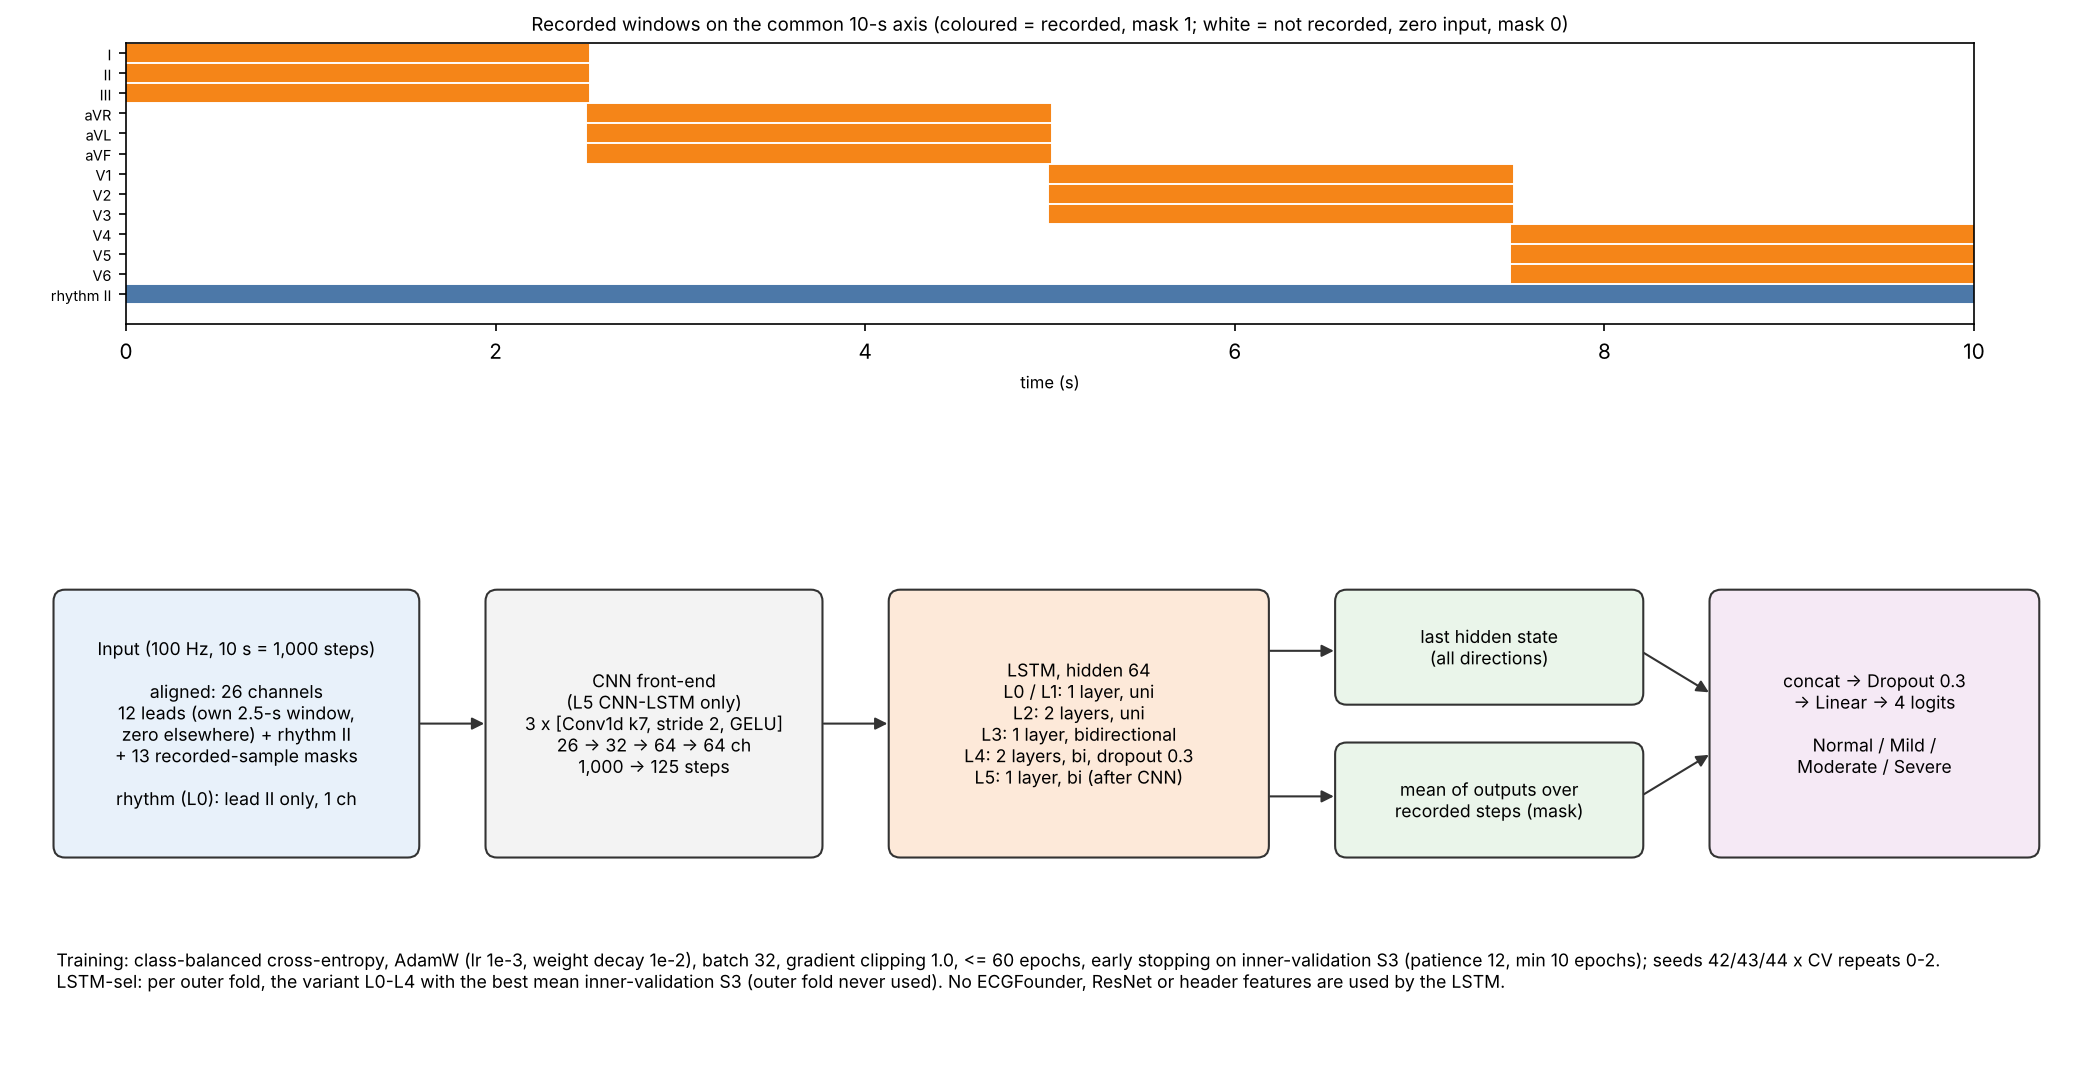
\includegraphics[width=0.95\linewidth]{figures/lstm_architecture.png}
\caption{Top: the printout gives each lead only its own 2.5-s column; only lead II covers 10 s. Bottom: the LSTM /
CNN-LSTM family tested in Phases 6A--6B.}\label{fig:lstm}
\end{figure}

\begin{table}[H]\centering\small
\caption{Phase 6A key results (original labels; corrected 95\,\% CI). ``Adm.'' means every class recall $\ge 0.15$.}\label{tab:p6a}
\begin{adjustbox}{max width=\linewidth}
\begin{tabular}{lccccc}\toprule
Model & Adm. & Accuracy [95\,\% CI] & Macro-F1 & Mild F1 & Mild recall \\\midrule
C3 Phase 5 selected & yes & 0.561 [0.520, 0.603] & 0.448 & 0.221 & 0.177 \\
C1 vote ensemble & yes & 0.547 [0.504, 0.590] & 0.455 & 0.255 & 0.220 \\
C2 calibrated MLP & no & 0.568 [0.534, 0.603] & 0.442 & 0.160 & 0.112 \\
ECGFounder fine-tuned (A1) & yes & 0.536 [0.492, 0.581] & 0.436 & 0.202 & 0.164 \\
ECGFounder frozen, linear & yes & 0.528 [0.484, 0.573] & 0.434 & 0.244 & 0.214 \\
C3 recipe [A270] & yes & 0.561 [0.518, 0.604] & 0.446 & 0.237 & 0.193 \\
C3 recipe [B2] & no & 0.554 [0.511, 0.596] & 0.434 & 0.187 & 0.142 \\
C3 recipe [B3] & no & 0.559 [0.518, 0.600] & 0.426 & 0.144 & 0.103 \\
LSTM L0 (rhythm only) & no & 0.426 [0.387, 0.466] & 0.257 & 0.065 & 0.040 \\
LSTM L2 (best single) & no & 0.483 [0.437, 0.529] & 0.352 & 0.114 & 0.076 \\
LSTM-sel (nested) & no & 0.470 [0.424, 0.515] & 0.344 & 0.122 & 0.081 \\
CNN-LSTM L5 & yes & 0.484 [0.435, 0.532] & 0.368 & 0.219 & 0.191 \\\bottomrule
\end{tabular}
\end{adjustbox}
\end{table}
\textbf{Findings:}
\begin{itemize}
  \item Mild is the main difficulty. Of 185 Mild ECGs, C3 predicts 79 as Normal, 52 as Moderate and 21 as Severe, and
    only 33 as Mild.
  \item A270, B2 and B3 give no improvement (all Holm $p=1.00$). The apparent B2 gain on B2 labels is a
    \emph{definition effect}, not a training effect.
  \item The only significant results are the \emph{inferiority} of the standalone LSTMs (about $-0.09$ accuracy vs C3).
\end{itemize}

% ---------------------------------------------------------------------------------------------------------
\section{Phase 6B: EF thresholds, Normal training size and the LSTM family}\label{sec:p6b}
\textbf{Goal.}
\begin{itemize}
  \item Clinically motivated threshold variants: T50 (Normal $\ge50$\,\%) and T55 (Normal $\ge55$\,\%).
  \item Normal training sizes 300 / 270 / 240 / 200.
  \item Removal of uncertain cases (XUNC).
  \item CNN-LSTM with and without the header, and early or late fusion with ECGFounder.
\end{itemize}
Branch \texttt{research/phase6}, folder \texttt{phase\_6b\_threshold\_sampling\_lstm}.

\begin{table}[H]\centering\small
\caption{Phase 6B: existing recipe under each configuration, scored on the \emph{original} labels (accuracy / Mild recall).}\label{tab:p6b}
\begin{adjustbox}{max width=\linewidth}
\begin{tabular}{lcccc}\toprule
Config & MLP fusion & C1 vote & C3 & LSTM-fixed \\\midrule
ORIG & 0.544 / 0.141 & 0.548 / 0.222 & 0.562 / 0.178 & 0.467 / 0.067 \\
T50 & 0.548 / 0.148 & 0.547 / 0.205 & 0.554 / 0.142 & 0.466 / 0.068 \\
T55 & 0.544 / 0.166 & 0.544 / 0.207 & \textbf{0.569} / 0.186 & 0.459 / 0.097 \\
XUNC & 0.545 / 0.124 & 0.542 / 0.169 & 0.559 / 0.103 & 0.462 / 0.077 \\
N300 & 0.546 / 0.142 & 0.543 / 0.220 & 0.559 / 0.184 & 0.464 / 0.068 \\
N270 & 0.545 / 0.142 & 0.547 / 0.225 & 0.558 / 0.195 & 0.458 / 0.086 \\
N240 & 0.539 / 0.155 & 0.545 / 0.227 & 0.558 / 0.209 & 0.474 / 0.072 \\
N200 & 0.541 / 0.150 & 0.546 / 0.234 & 0.553 / 0.220 & 0.470 / 0.067 \\\bottomrule
\end{tabular}
\end{adjustbox}
\end{table}

\begin{table}[H]\centering\small
\caption{Phase 6B LSTM family and fusions (original labels).}\label{tab:p6b2}
\begin{adjustbox}{max width=\linewidth}
\begin{tabular}{lccccc}\toprule
Model & Accuracy [95\,\% CI] & Macro-F1 & Mild recall & Parameters & Train min/run \\\midrule
F4 vote + LSTM-sel + prior rule & 0.559 [0.517, 0.600] & 0.449 & 0.182 & C1 + 24k--147k & 3.52 \\
F3 vote + LSTM-sel & 0.553 [0.508, 0.597] & 0.453 & 0.198 & C1 + 24k--147k & 2.29 \\
F2 CNN-LSTM + header + f6 & 0.551 [0.517, 0.585] & 0.452 & 0.166 & 198,820 & 0.26 \\
F1 LSTM-fixed + header + f6 & 0.540 [0.507, 0.573] & 0.439 & 0.151 & 130,372 & 0.29 \\
L6 CNN-LSTM + header & 0.497 [0.456, 0.539] & 0.389 & 0.182 & 116,644 & 0.27 \\
L5 CNN-LSTM & 0.484 [0.435, 0.532] & 0.368 & 0.191 & 116,580 & 0.38 \\
LSTM-fixed L3 & 0.467 [0.417, 0.516] & 0.337 & 0.067 & 48,132 & 0.44 \\\bottomrule
\end{tabular}
\end{adjustbox}
\end{table}
\textbf{Findings:}
\begin{itemize}
  \item No configuration or fusion improves on C3; all Holm $p=1.00$. T55 training gives the highest admissible
    figure on original labels (0.569), but $+0.007$ is not significant.
  \item Reducing Normal training ECGs shifts the prior (Mild recall rises, Normal recall falls) without better
    discrimination (Figure~\ref{fig:nsize}).
  \item Under T50 the higher scores are a definition effect: 27 hard borderline Mild ECGs become Normal.
\end{itemize}

\begin{figure}[H]\centering
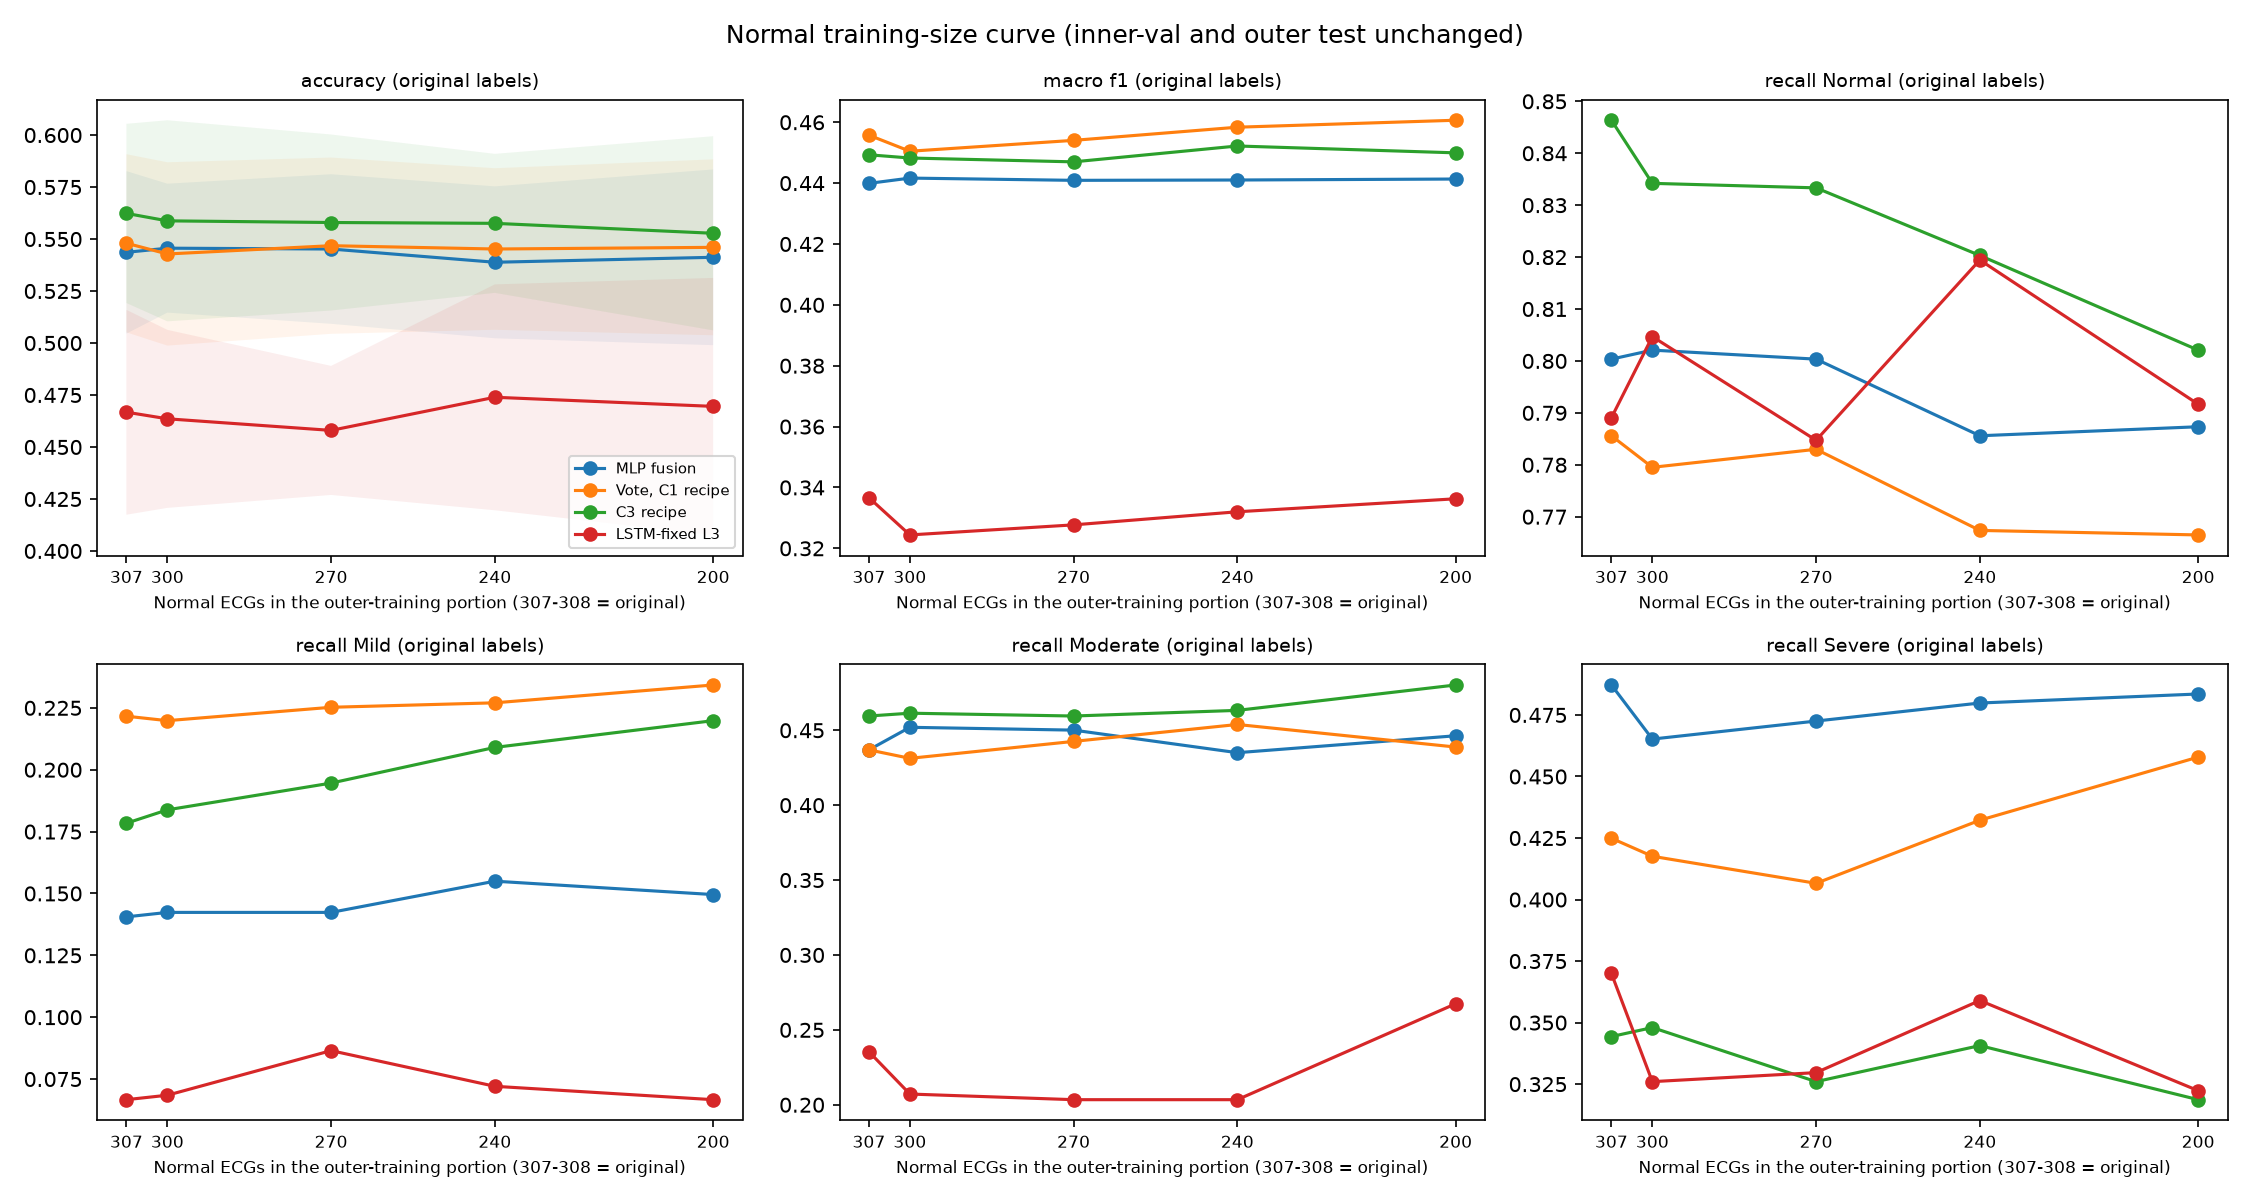
\includegraphics[width=0.7\linewidth]{figures/normal_size_curve.png}
\caption{Normal training size vs accuracy and recall (Phase 6B).}\label{fig:nsize}
\end{figure}

% ---------------------------------------------------------------------------------------------------------
\section{Label-quality and cohort studies (exploratory)}\label{sec:labels}
These studies answered the owner's questions about hard borderline cases, label cleaning and ``reliable'' subsets.
All are on branch \texttt{research/phase6} (\texttt{phase\_6b\_threshold\_sampling\_lstm/}), each with a dated
amendment written before it was run.

\begin{table}[H]\centering\small
\caption{Label / cohort studies. Accuracy on all 837 ECGs unless stated.}\label{tab:labels}
\begin{adjustbox}{max width=\linewidth}
\begin{tabular}{p{4.4cm}p{4.6cm}p{5.4cm}}\toprule
Study & Result & Conclusion \\\midrule
VER: 15 labels corrected to a high-confidence echo & C3 0.565 (+0.004) & label noise explains $<$\,1 point \\
VERB / BRES: resolve or remove borderline cases & gains only by abandoning Mild & not admissible \\
CLEAR: train without border cases & 0.548 all; 0.668 on clear-cut; Mild recall 0.13 & subset gain, not a model gain \\
SUB591: N 200 / Mi 150 / Mo 150 / S all & 0.548 all; 0.489 on subset & no gain \\
HC30: train and test on 395 exact-name, $\le$\,30-day links & 0.594 (C3 trained on all: 0.598) & reliable labels alone do not help \\
HC30F: + all ECG factor families & 0.603 on HC30 (Mild recall 0.25) & $+0.005$, noise level \\
MMCLEAN: remove suspect Mild/Moderate (217) & 0.547 all; 0.677 on kept 620 (Mild recall 0.09) & higher numbers come from easier subsets \\
NF / NFS: noise-free training & 0.546 / 0.552 all; C3 0.707 on 264 clean, clear-cut & cleaning does not raise all-ECG accuracy \\
MILDFIX F1--F3: Mild-aware, ordinal, EF-based rules & 0.537--0.560 & trade accuracy for Mild \\
Circularity check: relabel border cases to model output & 0.764, but random guessing also rises 0.244 $\to$ 0.470 & \textbf{invalid} (circular); excluded \\\bottomrule
\end{tabular}
\end{adjustbox}
\end{table}
\textbf{Selective prediction} (answer only above a nested confidence threshold) first reached about 0.71 on 22\,\% of
ECGs (MMCLEAN, Figure~\ref{fig:coverage}). It was refined in Phase 7 into the final triage model (Section~\ref{sec:final}).

\begin{figure}[H]\centering
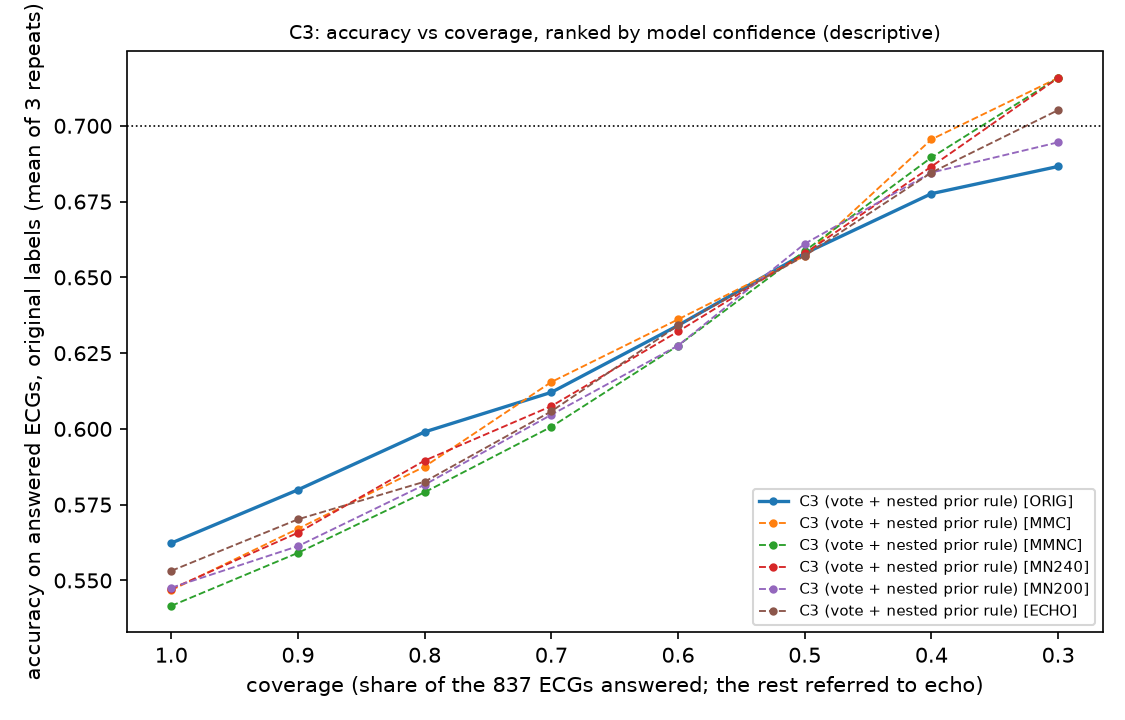
\includegraphics[width=0.62\linewidth]{figures/mmclean_coverage_curve.png}
\caption{Accuracy vs share of ECGs answered (selective prediction).}\label{fig:coverage}
\end{figure}

% ---------------------------------------------------------------------------------------------------------
\section{Phase 7: representation and head experiments, learning curve, triage}\label{sec:p7}
\textbf{Branches:} \texttt{research/phase6} (\texttt{phase\_7/}) and \texttt{research/phase7-testkit} (frozen
model and locked test). \textbf{Pilot gate:} accuracy $\ge +0.010$ or Mild F1 $\ge +0.03$, with macro-F1
$\ge -0.010$. No candidate passed (Table~\ref{tab:p7}).

\begin{table}[H]\centering\small
\caption{Phase 7 pilots (seed 42, 3 repeats).}\label{tab:p7}
\begin{adjustbox}{max width=\linewidth}
\begin{tabular}{llccc}\toprule
Exp. & Candidate & Accuracy & Macro-F1 & Mild P / R / F1 \\\midrule
ref & MLP fusion [header $\|$ f6] & 0.544 & 0.436 & 0.283 / 0.132 / 0.179 \\
E1 & stage-5 mean $\|$ max $\|$ std & 0.517 & 0.409 & 0.263 / 0.146 / 0.187 \\
E1 & per-printed-column stage-5 mean & 0.527 & 0.431 & 0.271 / 0.157 / 0.199 \\
E1 & stage-4 mean $\|$ f6 (multi-scale) & 0.529 & 0.425 & 0.250 / 0.141 / 0.178 \\
E1 & 150 ECGFounder diagnostic outputs & 0.531 & 0.412 & 0.287 / 0.117 / 0.165 \\
E2 & multitask CE + verified-EF regression & 0.545 & 0.440 & 0.289 / 0.142 / 0.191 \\
E2 & boundary-aware soft labels & 0.548 & 0.433 & 0.303 / 0.123 / 0.174 \\
E2 & EF-weighted supervised contrastive & 0.546 & 0.436 & 0.276 / 0.130 / 0.176 \\
E3 & multi-lead 1-D ResNet (repeat 0) & 0.496 & 0.384 & 0.264 / 0.178 / 0.213 \\
E3 & 1-D ResNet + header (repeat 0) & 0.485 & 0.378 & 0.243 / 0.189 / 0.213 \\\bottomrule
\end{tabular}
\end{adjustbox}
\end{table}

\paragraph{E5: learning curve} (Figure~\ref{fig:lc}):
\begin{itemize}
  \item each doubling of training data gives $+1.4$ accuracy points, with no trend in Mild F1;
  \item the EF error SD falls by 0.44 points per doubling (0.66 on verified-EF ECGs);
  \item extrapolation: about $10^5$ ECGs of current label quality would give about 0.65.
\end{itemize}

\begin{figure}[H]\centering
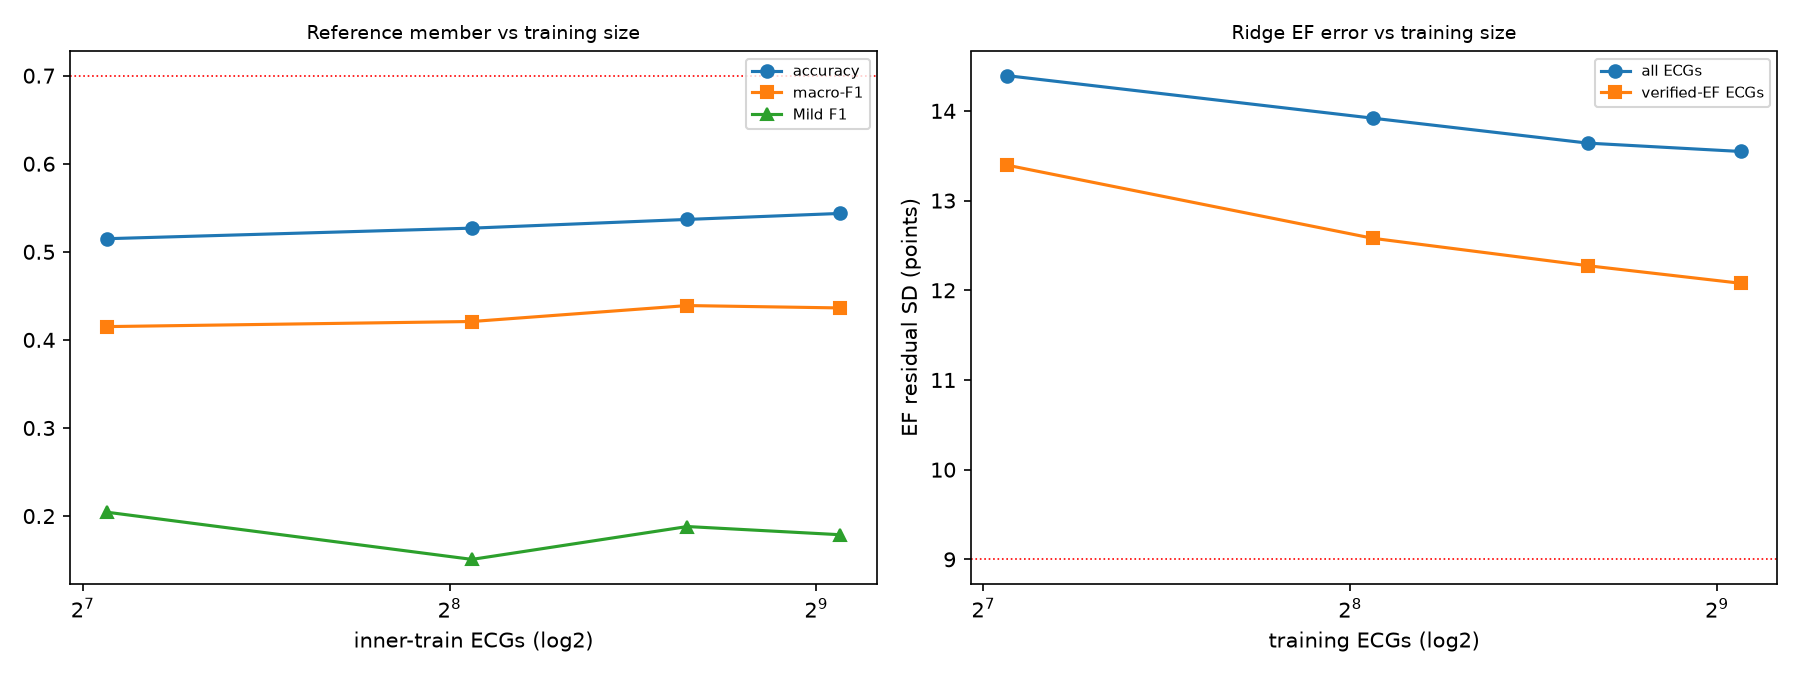
\includegraphics[width=0.95\linewidth]{figures/phase7_learning_curve.png}
\caption{Phase 7 learning curve: classification metrics (left) and EF error (right) vs training size.}\label{fig:lc}
\end{figure}

\paragraph{E6: header-free cascades.}
\begin{itemize}
  \item EF-grading stage 1 alone: 0.693 on 53\,\% answered (G2T-img); 0.694 on 56\,\% when it must agree with IMG-C3
    (AGT-img, the final triage).
  \item As complete four-class classifiers the cascades reach 0.548--0.568, no genuine gain.
  \item Stage 1 answers almost only Normal.
\end{itemize}

\paragraph{E7: Mild-aware selective prediction.}
\begin{itemize}
  \item Accuracy $\ge 0.70$ together with detecting $\ge 10$\,\% of Mild patients is \emph{infeasible} in all 15
    training folds.
  \item Even the most confident Mild calls are right only 20--50\,\% of the time.
\end{itemize}

% ---------------------------------------------------------------------------------------------------------
\section{Final push on image-only four-class accuracy}\label{sec:push}
At the owner's request (image only, Mild $\ge 15$\,\%), four further pre-registered studies were run. They are on
branch \texttt{research/phase6}: \texttt{HIER\_REPORT.md}, \texttt{ENH\_REPORT.md}, \texttt{ULT\_REPORT.md} and
\texttt{ECHONEXT\_REPORT.md}.

\begin{table}[H]\centering\small
\caption{Image-only four-class models, all 837 ECGs (no header, age or sex input).}\label{tab:push}
\begin{adjustbox}{max width=\linewidth}
\begin{tabular}{p{6.2cm}cc}\toprule
Model & Accuracy [95\,\% CI] & Recall N / Mi / Mo / S \\\midrule
HIER: two-stage (N / middle / S, then Mi vs Mo) & 0.558 [0.522, 0.594] & 0.86 / 0.17 / 0.41 / 0.34 \\
HIER-ext (wider tuning grid) & 0.570 [0.527, 0.612] & 0.88 / 0.16 / 0.43 / 0.34 \\
ENH: synth 10-s reconstruction $\to$ ECGFounder (M2) & 0.528 & 0.76 / 0.18 / 0.44 / 0.41 \\
ENH: same head on aligned input (D1 reference) & 0.537 & 0.78 / 0.21 / 0.41 / 0.42 \\
ENH: median-beat shape (M3) & 0.467 & 0.68 / 0.19 / 0.36 / 0.33 \\
ENH: MiniRocket (M4) & 0.504 & 0.74 / 0.22 / 0.38 / 0.33 \\
ENH: EF-ordinal ridge (M6) & 0.534 & 0.95 / 0.29 / 0.00 / 0.29 \\
ENH-vote (6 members, tuned class weights) & 0.569 [0.527, 0.610] & 0.88 / 0.17 / 0.46 / 0.29 \\
\textbf{ULT-stack (10 members + predicted EF)} & \textbf{0.571 [0.542, 0.600]} & 0.91 / 0.16 / 0.42 / 0.29 \\
ULT2-stack (+ EchoNext-Mini external model) & 0.569 [0.538, 0.599] & 0.90 / 0.15 / 0.44 / 0.28 \\
EchoNext-Mini outputs + LR alone & 0.486 [0.436, 0.536] & 0.72 / 0.11 / 0.36 / 0.53 \\\bottomrule
\end{tabular}
\end{adjustbox}
\end{table}
\textbf{Findings:}
\begin{itemize}
  \item \textbf{Two-stage:} stage 1 (Normal / middle / Severe) is right 66--67\,\% of the time. Stage 2 (Mild vs
    Moderate) is right only 53--58\,\%, close to a coin flip.
  \item \textbf{Reconstruction:} a faithful beat-synchronous 10-s 12-lead reconstruction (template $r=0.98$) adds
    no EF information.
  \item \textbf{External knowledge:} EchoNext-Mini (Hughes et al., 2026; Poterucha et al., 2025), trained on about
    100,000 US patients, transfers to the printouts (AUROC 0.79 for EF $\le 45$\,\%). It is weaker than the in-house
    EF model (0.86) and adds no accuracy.
  \item \textbf{Ensembles:} all ensembles plateau at $0.57\pm0.01$ (Figure~\ref{fig:landscape}).
\end{itemize}

% ---------------------------------------------------------------------------------------------------------
\section{Sensitivity to the class definition (band sweep)}\label{sec:bands}
\begin{itemize}
  \item \textbf{Sweep:} 3,313 definitions (Normal limit 45--56, Mild/Moderate 35--46, Moderate/Severe 25--36, sex
    offset 0/2) were evaluated with one header-free EF model. 1,457 of them are feasible (every class $\ge 60$
    ECGs, both middle bands $\ge 5$ points wide).
  \item \textbf{Confirmation:} the selected definitions were retrained.
  \item \textbf{Result:} the clinically pre-specified \textbf{ESC 2021} definition (Normal $\ge 50$, Mild 41--49,
    Moderate 30--40, Severe $<30$) gives \textbf{0.626 [0.588, 0.664]} with every class detected (Mild 17\,\%,
    Moderate 42\,\%).
  \item \textbf{Trade-off:} no definition detects both Mild and Moderate well (Figure~\ref{fig:bands}).
\end{itemize}
These figures belong to a different task definition and are reported only as a sensitivity analysis.

\begin{table}[H]\centering\small
\caption{Confirmed band definitions (retrained header-free vote).}\label{tab:bands}
\begin{adjustbox}{max width=\linewidth}
\begin{tabular}{lcccc}\toprule
Definition & N / Mi / Mo / S ECGs & Accuracy [95\,\% CI] & $\kappa$ & Detected N / Mi / Mo / S \\\midrule
Original limits on echo EF & 415 / 170 / 165 / 87 & 0.594 [0.560, 0.627] & 0.353 & 91 / 20 / 32 / 38\,\% \\
\textbf{ESC 2021} & 446 / 139 / 176 / 76 & \textbf{0.626} [0.588, 0.664] & 0.384 & 90 / 17 / 42 / 35\,\% \\
Best Mild detection ($>$51 / 38 / 31) & 439 / 197 / 114 / 87 & 0.619 [0.593, 0.645] & 0.380 & 90 / 28 / 25 / 43\,\% \\
Best $\kappa$ ($>$52 / 46 / 29) & 428 / 70 / 272 / 67 & 0.634 [0.591, 0.678] & 0.399 & 87 / 12 / 49 / 27\,\% \\\bottomrule
\end{tabular}
\end{adjustbox}
\end{table}

\begin{figure}[H]\centering
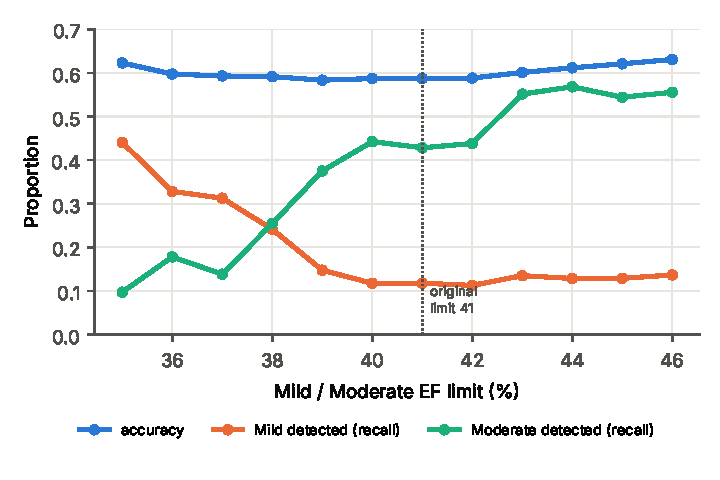
\includegraphics[width=0.62\linewidth]{figures/fig_band_sweep.pdf}
\caption{Moving the Mild/Moderate limit trades Mild detection against Moderate detection.}\label{fig:bands}
\end{figure}

% ---------------------------------------------------------------------------------------------------------
\section{Why accuracy plateaus at about 0.57 on all patients}\label{sec:why}
More than 15 model families, 8 label-cleaning schemes, an external model trained on about 100,000 patients, and 3,313
class definitions all land at 0.55--0.57 four-class accuracy (0.63 with the ESC 2021 limits). The convergence points
to a limit in the \emph{information} carried by these printouts and labels, not in the modelling. The evidence:

\begin{enumerate}
  \item \textbf{EF precision vs band width.}
    \begin{itemize}
      \item The best header-free models estimate EF with $r\approx0.66$, residual SD about 13 points and MAE about 10.
      \item The Mild band (41 to 52/54) is about 12 points wide and the Moderate band 10.
      \item A simulation (true EF plus Gaussian error, cut at the class limits) gives an accuracy ceiling of 0.63 at
        SD 13. Reaching 0.73 needs SD 8, and 0.82 needs SD 5.
      \item The models reach 0.57--0.59, close to this ceiling.
    \end{itemize}
  \item \textbf{Errors sit at the class limits} (Figure~\ref{fig:boundary}).
    \begin{itemize}
      \item 51\,\% of ECGs have an echo EF within 6 points of a limit; their error rate is 62--68\,\%.
      \item ECGs at least 10 points from every limit are classified with 79--84\,\% accuracy.
      \item That clear-cut set contains no in-band Mild or Moderate ECG: those bands are too narrow.
    \end{itemize}
  \item \textbf{The ECG separates the extremes, not neighbouring grades.}
    \begin{itemize}
      \item Pairwise AUROC: Normal vs Severe 0.90 and Normal vs Moderate 0.88, but Normal vs Mild 0.75, Mild vs
        Moderate 0.63 and Moderate vs Severe 0.64.
      \item The best single Mild-vs-Moderate factor reaches 0.64.
      \item Mild differs from Normal mainly by conduction markers: QRS width, LBBB patterns.
    \end{itemize}
  \item \textbf{Label uncertainty.}
    \begin{itemize}
      \item EF comes from Teichholz M-mode reports.
      \item The echo is linked to the ECG by fuzzy name matching: only 44\,\% of ECGs have a clean link (exact name,
        echo within 30 days). 391 have a name-match score $<100$ and 192 an echo more than 30 days away.
      \item Repeat echoes of the same ECG differ by a median of 15.4 points (an upper bound).
      \item ECG--echo agreement is $r=0.75$ for clean links vs 0.42 for echoes more than 30 days away.
      \item Cleaning the labels changes all-ECG accuracy by only $-0.02$ to $+0.01$, because the remaining noise
        still exceeds the band width.
    \end{itemize}
  \item \textbf{Input format.}
    \begin{itemize}
      \item The PDFs give 2.5\,s per lead in four successive columns; only lead II covers 10 s.
      \item Foundation models were pre-trained on simultaneous 10-s digital ECGs.
      \item Reconstruction, multi-scale and per-column embeddings did not help. Digitisation quality was unrelated
        to error.
    \end{itemize}
  \item \textbf{Sample size.} 837 development ECGs, of which 185 are Mild. The learning curve gives $+1.4$ points per
    doubling, with no Mild trend.
\end{enumerate}

\begin{figure}[H]\centering
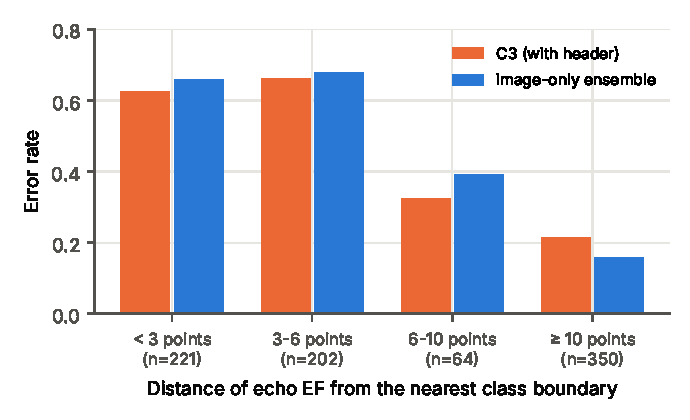
\includegraphics[width=0.62\linewidth]{figures/fig_error_vs_boundary.pdf}
\caption{Error rate by distance of the echo EF from the nearest class limit (all 837 ECGs, mean of 3 repeats).}\label{fig:boundary}
\end{figure}

\begin{figure}[H]\centering
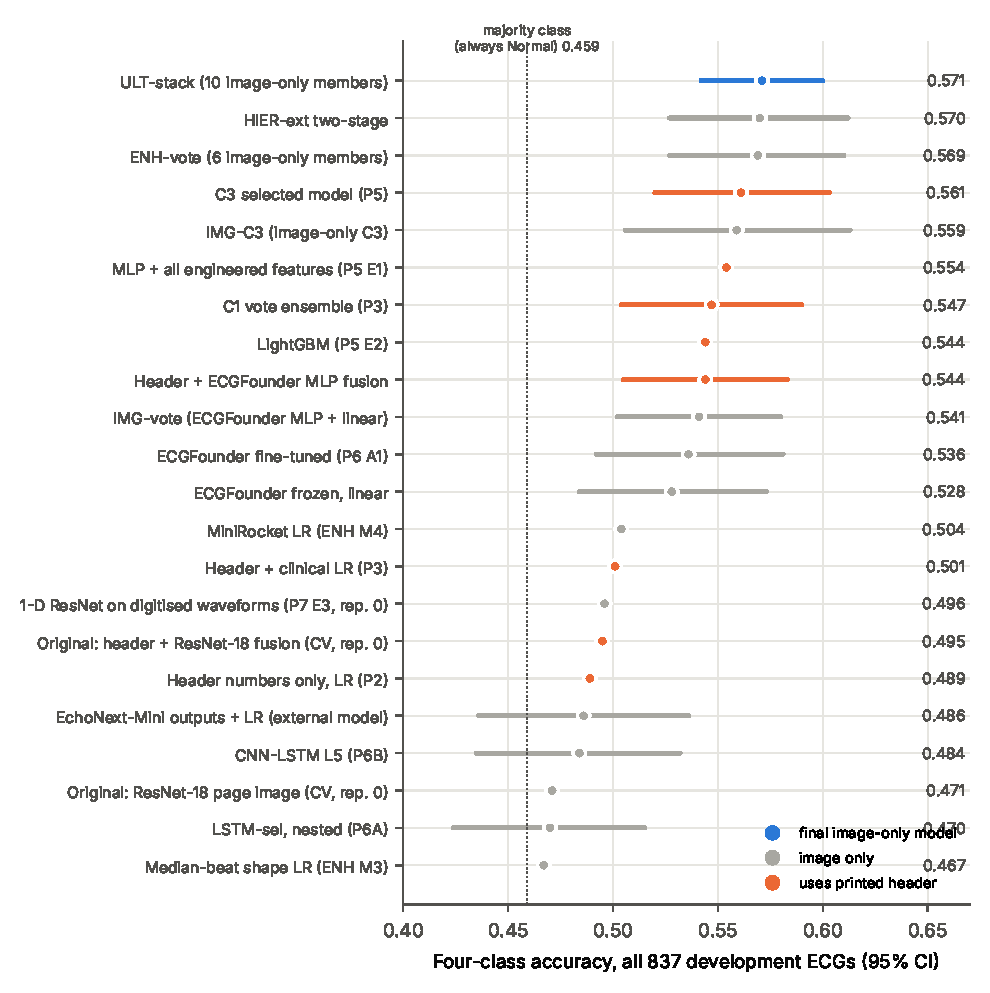
\includegraphics[width=0.92\linewidth]{figures/fig_model_landscape.pdf}
\caption{Four-class accuracy (all 837 development ECGs) of the main models across all phases. Image-only and
header-using models converge at 0.55--0.57.}\label{fig:landscape}
\end{figure}

% ---------------------------------------------------------------------------------------------------------
\section{Recommendations and ongoing work}\label{sec:future}
\begin{enumerate}
  \item \textbf{Verified ECG--echo linkage.} Link by MRN/UHID, with the echo within days and ideally in the same
    admission. A prioritised re-check worklist (197 high-priority ECGs, mostly Mild and Moderate) and a fill-in
    template are ready. A pipeline re-trains and re-scores the model as soon as verified data return; its self-test
    reproduces the current result exactly (\texttt{fixes.py}).
  \item \textbf{Biplane Simpson EF} instead of Teichholz, with repeat reads near the 41\,\% and 50--54\,\% limits.
  \item \textbf{Digital 10-s simultaneous ECGs} (XML/DICOM exports from the ECG machine) instead of PDF printouts.
  \item \textbf{More patients, enriched for Mild and Moderate.} At least 3,000 pairs, with at least 600 each of Mild
    and Moderate, preferably from a second centre.
  \item \textbf{Public-data pre-training (in progress, branch \texttt{research/public-ef}).}
    \begin{itemize}
      \item EchoNext (PhysioNet, credentialed) provides 100,000 ECGs with a numeric LVEF.
      \item Its ECGs are cut into the hospital printout layout, labelled with the same four-class rule, used for
        training, and then evaluated on the 837 development ECGs with the same folds.
      \item The data stay on the owner's laptop under the data-use agreement.
    \end{itemize}
  \item \textbf{A new prospective test set} scored once with the frozen test kit (\texttt{research/phase7-testkit}),
    because the locked set has now been used.
\end{enumerate}

% ---------------------------------------------------------------------------------------------------------
\appendix
\section{Repository branch map}\label{app:branches}
\begin{table}[H]\centering\small
\begin{adjustbox}{max width=\linewidth}
\begin{tabular}{p{4.6cm}p{10.4cm}}\toprule
Branch & Content \\\midrule
\url{main}, \url{claude/funny-gauss-udlmv0} & Original project: PDF preprocessing and baseline image models (code on \url{main}; results and write-up on \url{claude/funny-gauss-udlmv0}) \\
\url{research/ecg-ef-model-improvements} & Phases 1--3: improved models, Phase 3 report, \texttt{FINAL\_REPORT.md} \\
\url{research/phase4-handoff} & Phase 4: label quality, regression, multitask, final report \\
\url{research/phase5} & Phase 5: baselines, feature families, nested decision rules; selection of C3 \\
\url{research/phase6} & Phase 6 (foundation-model improvement), 6A, 6B and all exploratory studies; Phase 7 (\texttt{phase\_7/}); this report (\texttt{final\_report/}) \\
\url{research/phase7-testkit} & Frozen header-free triage model, test kit and the one-time locked-test result \\
\url{research/public-ef} & EchoNext public-data pre-training study (code only; data stay on the laptop) \\\bottomrule
\end{tabular}
\end{adjustbox}
\end{table}

\section{Glossary}\label{app:glossary}
\begin{description}
  \item[C1] Equal-weight vote of three members: the MLP fusion of the printed header and the ECGFounder embedding, an
    ECGFounder linear head (distance-penalised cross-entropy), and a header + clinical logistic regression.
  \item[C2] Calibrated MLP fusion (not admissible: Mild recall 0.11).
  \item[C3] C1 plus a class-prior decision rule tuned inside the training folds. The Phase 5 selected model.
  \item[IMG-C3] The C3 recipe without any header input (ECGFounder heads only).
  \item[Admissible] Every class recall $\ge 0.15$.
  \item[Definition vs training effect] Under changed labels, the gain of the unchanged model (definition effect)
    vs the gain from retraining (training effect).
  \item[Aligned / synth input] The 12 $\times$ 10-s ECGFounder input built from the printout: leads at their true
    2.5-s position with zeros elsewhere (aligned), or a beat-synchronous reconstruction (synth).
  \item[Triage] A model that answers only when confident and otherwise refers to echocardiography.
\end{description}

\section{Integrity and reproducibility}\label{app:repro}
\begin{itemize}
  \item \textbf{Pre-registration:} every phase and exploratory study has a plan or a dated amendment committed
    \emph{before} it was run. Plan hashes are stored in \texttt{configs/PLAN.sha256}.
  \item \textbf{Locked test:} the 210-ECG test set was never used for training or selection. It was scored exactly
    once, with the owner's written authorisation, by the frozen model (2026-11-06; rules committed beforehand).
  \item \textbf{Privacy:} only aggregate metrics are committed. Per-ECG predictions, embeddings, model weights and
    the ECG--echo sheets stay in git-ignored folders, and every push is privacy-scanned.
  \item \textbf{Excluded as invalid:} relabelling ECGs to the model's own predictions (circular), and hand-picking
    evaluation cases.
  \item \textbf{Re-running a study:} each study's code is next to its report. For example:
{\footnotesize
\begin{verbatim}
python -m research_experiments.phase_6b_threshold_sampling_lstm.ult \
       --members --combine
python -m research_experiments.phase_7.testkit.score --help
python -m research_experiments.final_report.make_figures
\end{verbatim}}
\end{itemize}

\section*{References}
\begin{itemize}
  \item Li J, et al. An electrocardiogram foundation model built on over 10 million recordings (ECGFounder).
    \emph{NEJM AI}, 2025.
  \item McKeen K, et al. ECG-FM: an open electrocardiogram foundation model. \emph{JAMIA Open}, 2025.
  \item Hughes JW, Jing L, Finer J, et al. EchoNext-Mini: a dataset and baseline AI model for detecting structural
    heart disease from electrocardiograms. \emph{NEJM AI}, 2026. doi:10.1056/AIdbp2500516.
  \item Poterucha TJ, et al. Detecting structural heart disease from electrocardiograms using AI. \emph{Nature}, 2025;
    644(8075). doi:10.1038/s41586-025-09227-0.
  \item McDonagh TA, et al. 2021 ESC Guidelines for the diagnosis and treatment of acute and chronic heart failure.
    \emph{Eur Heart J}, 2021.
  \item Nadeau C, Bengio Y. Inference for the generalization error. \emph{Machine Learning}, 2003 (corrected
    resampled $t$-test).
  \item Dempster A, Schmidt DF, Webb GI. MiniRocket: a very fast (almost) deterministic transform for time series
    classification. \emph{KDD}, 2021.
\end{itemize}


\end{document}
